\documentclass[a4paper,12pt]{jsarticle}


% 数式
\usepackage{amsmath,amsfonts}
\usepackage{bm}
% 画像
\usepackage[dvipdfmx]{graphicx}



\begin{document}

\title{VScode Latex 覚書}
\author{早川悠介}
\date{\today}
\maketitle
iPad Proに描いたリンゴの絵を写真で撮り、画像表示のテストに用いる。
結構うまくかけていると思う。
複数のファイルがある場合にpdfができない問題は解決した。
bibtexがうまく働かない問題もsettings.jsonファイルを適切なものにし、ptex2pdf$\rightarrow$pbibtexとptex2pdf$\times 2$の二回に分けてコンパイルすることによって解決した。ほかに詰まった点としてはファイル名に拡張子前の"."以外にも"."が含まれるとなぜかうまくコンパイルできないことがあげられる。ファイル名が理由でうまくいかないとは思わなかったので覚えておこう。
.texファイルが変更されたときに自動的にコンパイルするようにもできる。.jsonファイルに記述しておくことで可能になる。

\begin{figure}[htbp]
\begin{center}
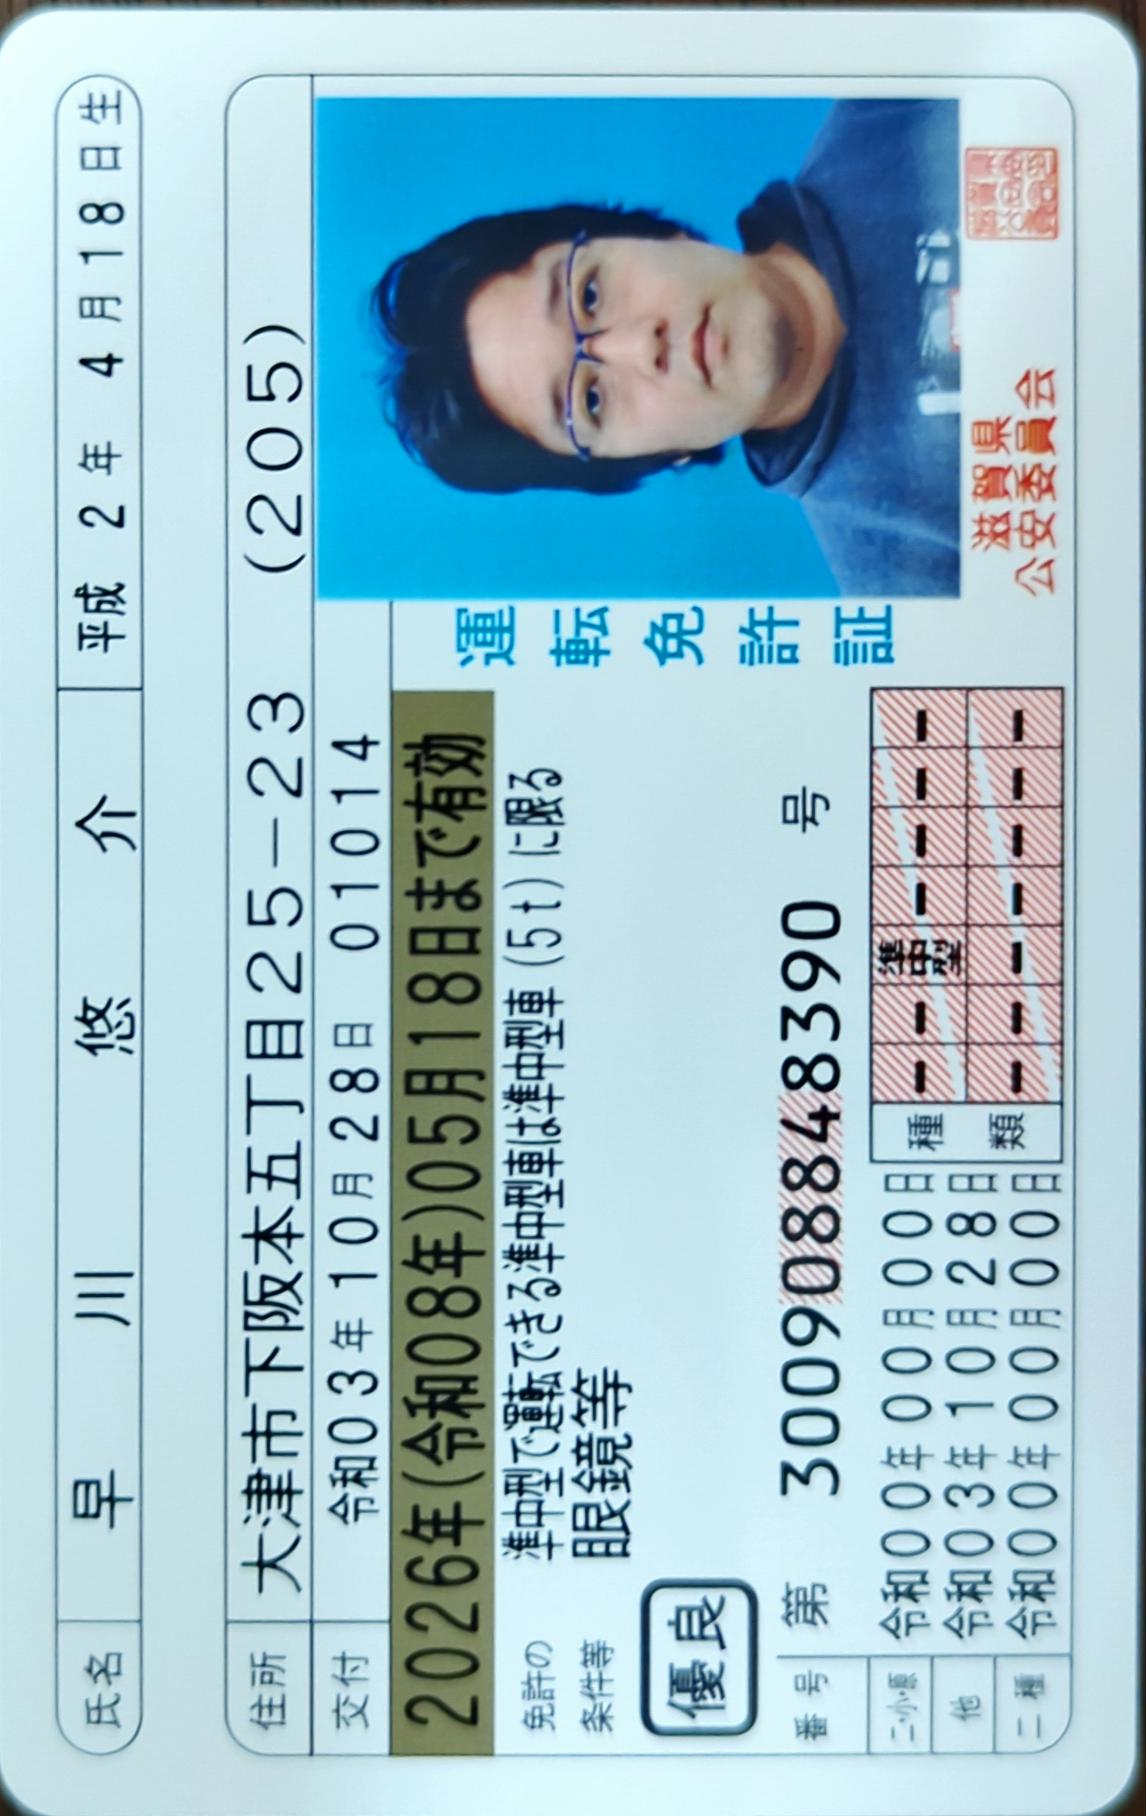
\includegraphics[width=60mm,angle=270]{2022_05_27_2.jpg}
\caption{Apple}
\end{center}
\end{figure}

\begin{figure}[htbp]
\begin{center}
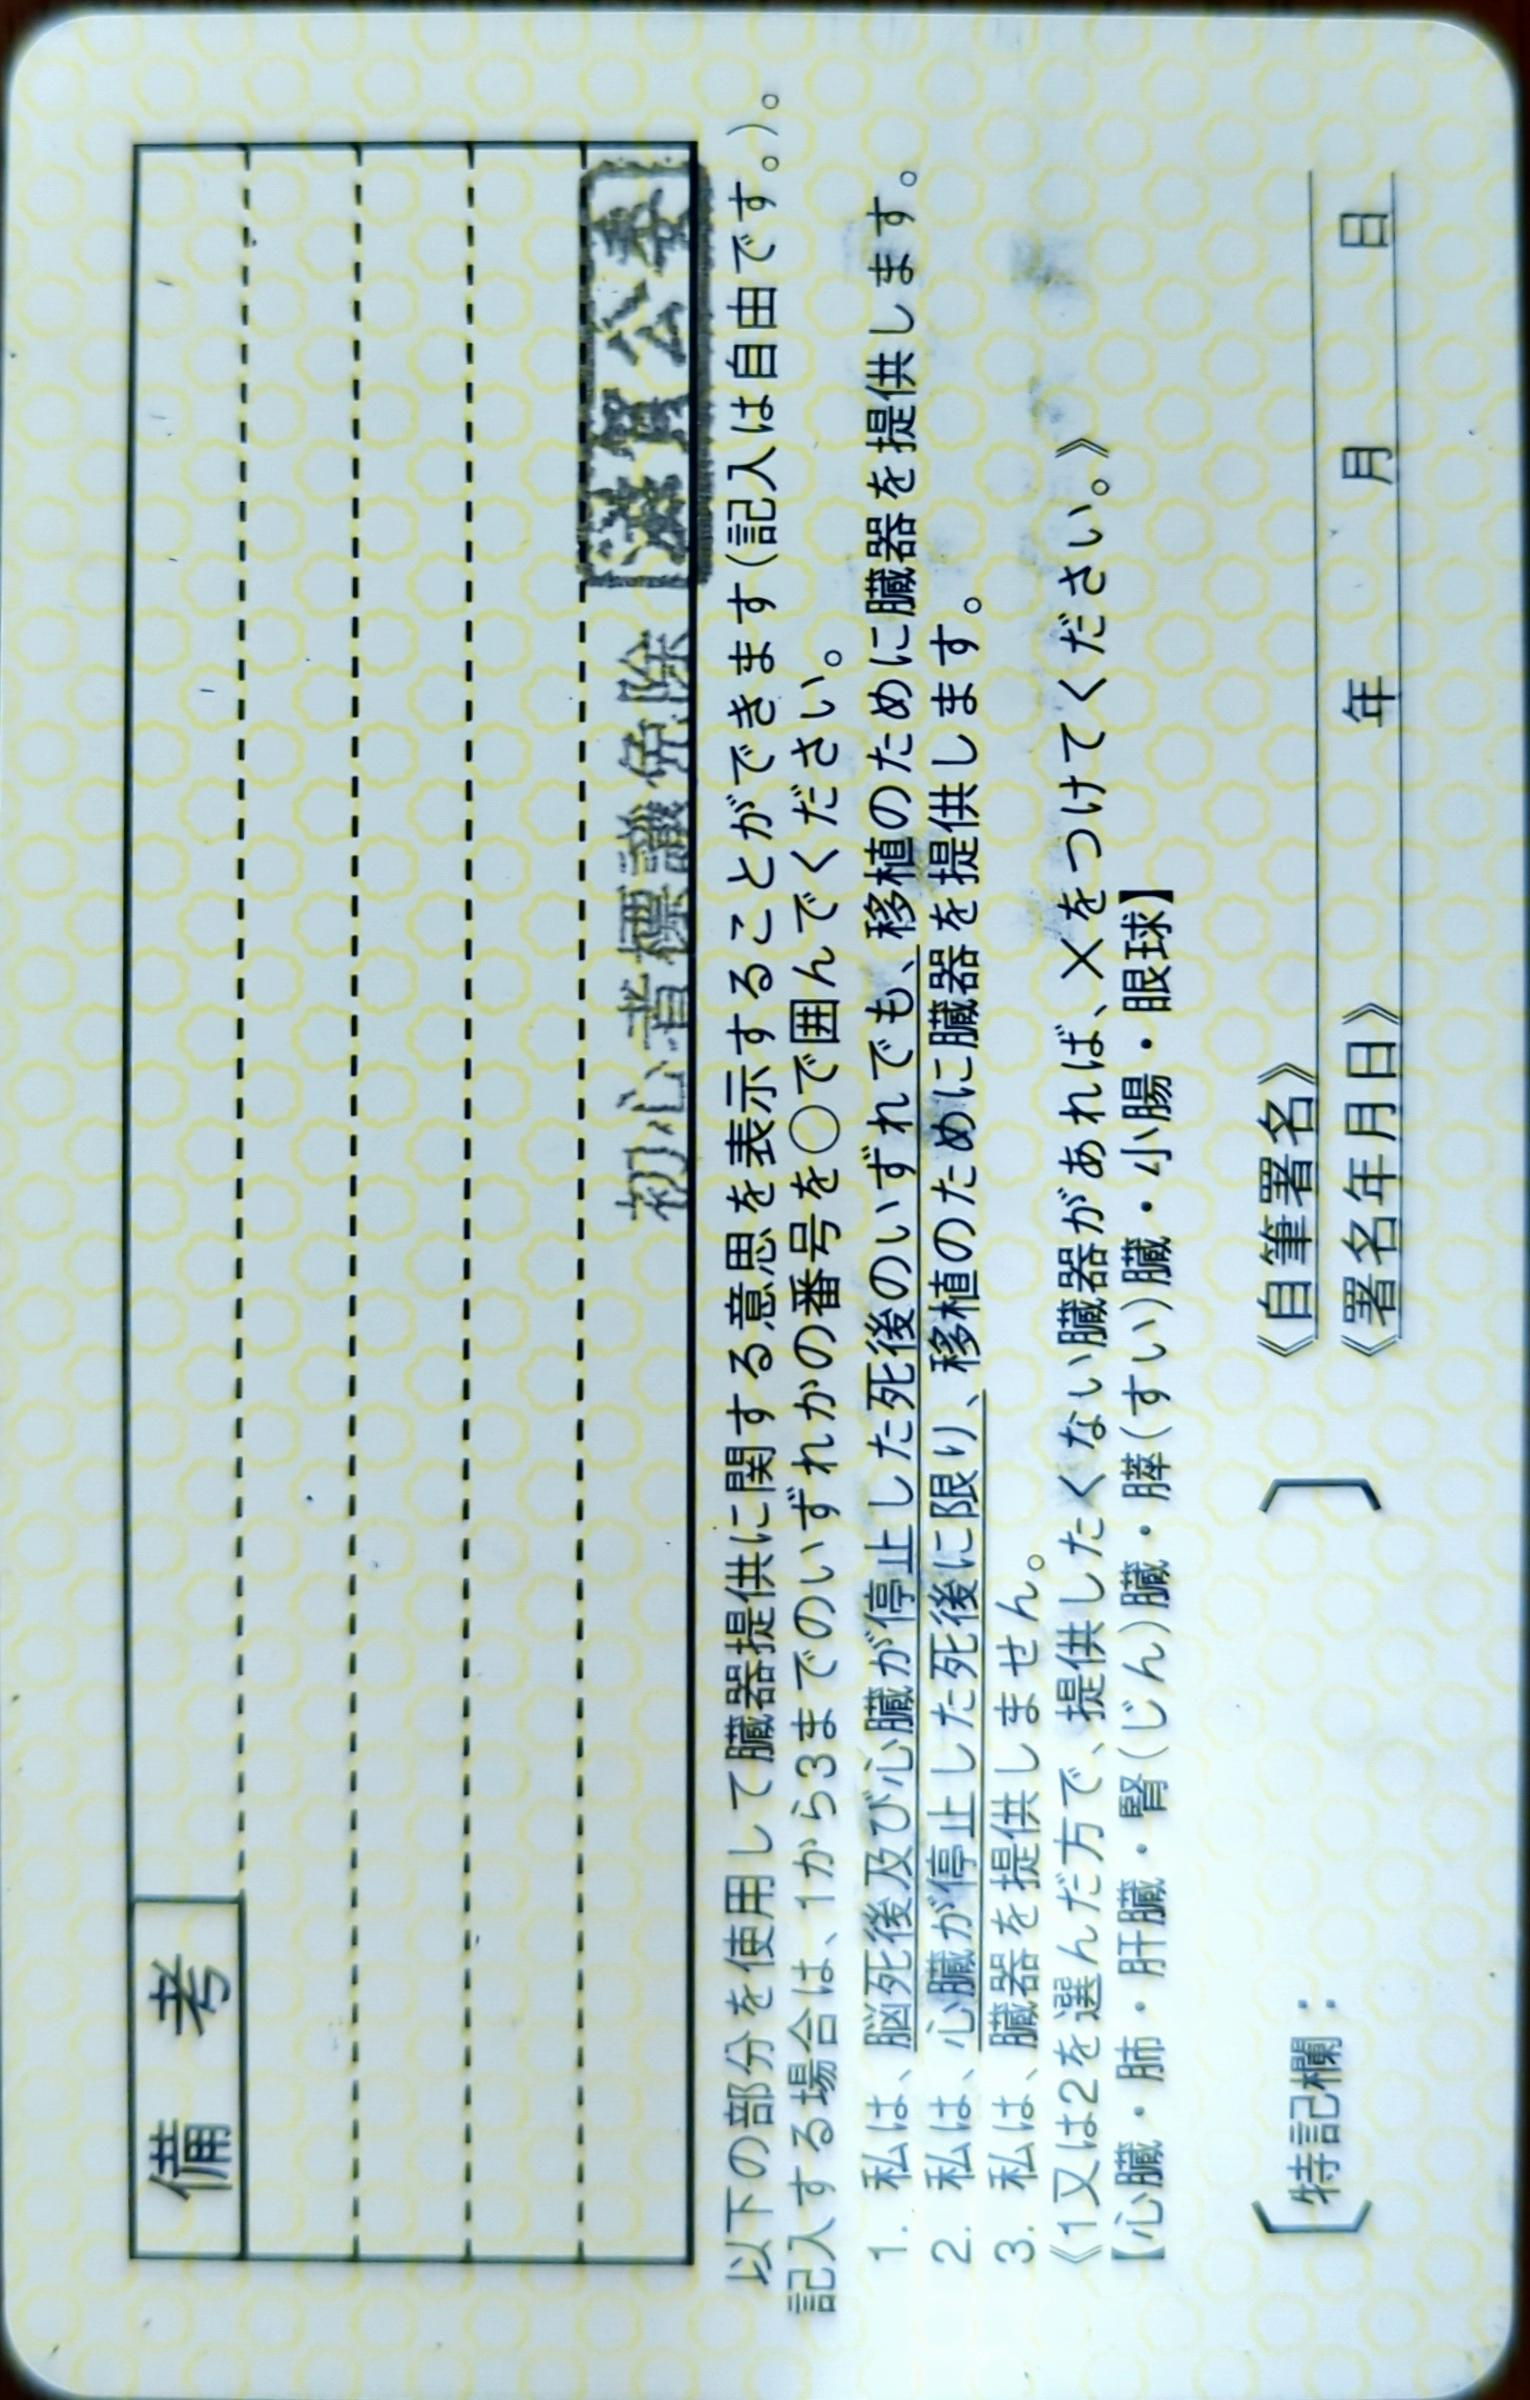
\includegraphics[width=60mm,angle=270]{2022_05_27_1.jpg}
\caption{Apple}
\end{center}
\end{figure}

\begin{figure}[htbp]
    \begin{minipage}[b]{0.45\linewidth}
      \centering
      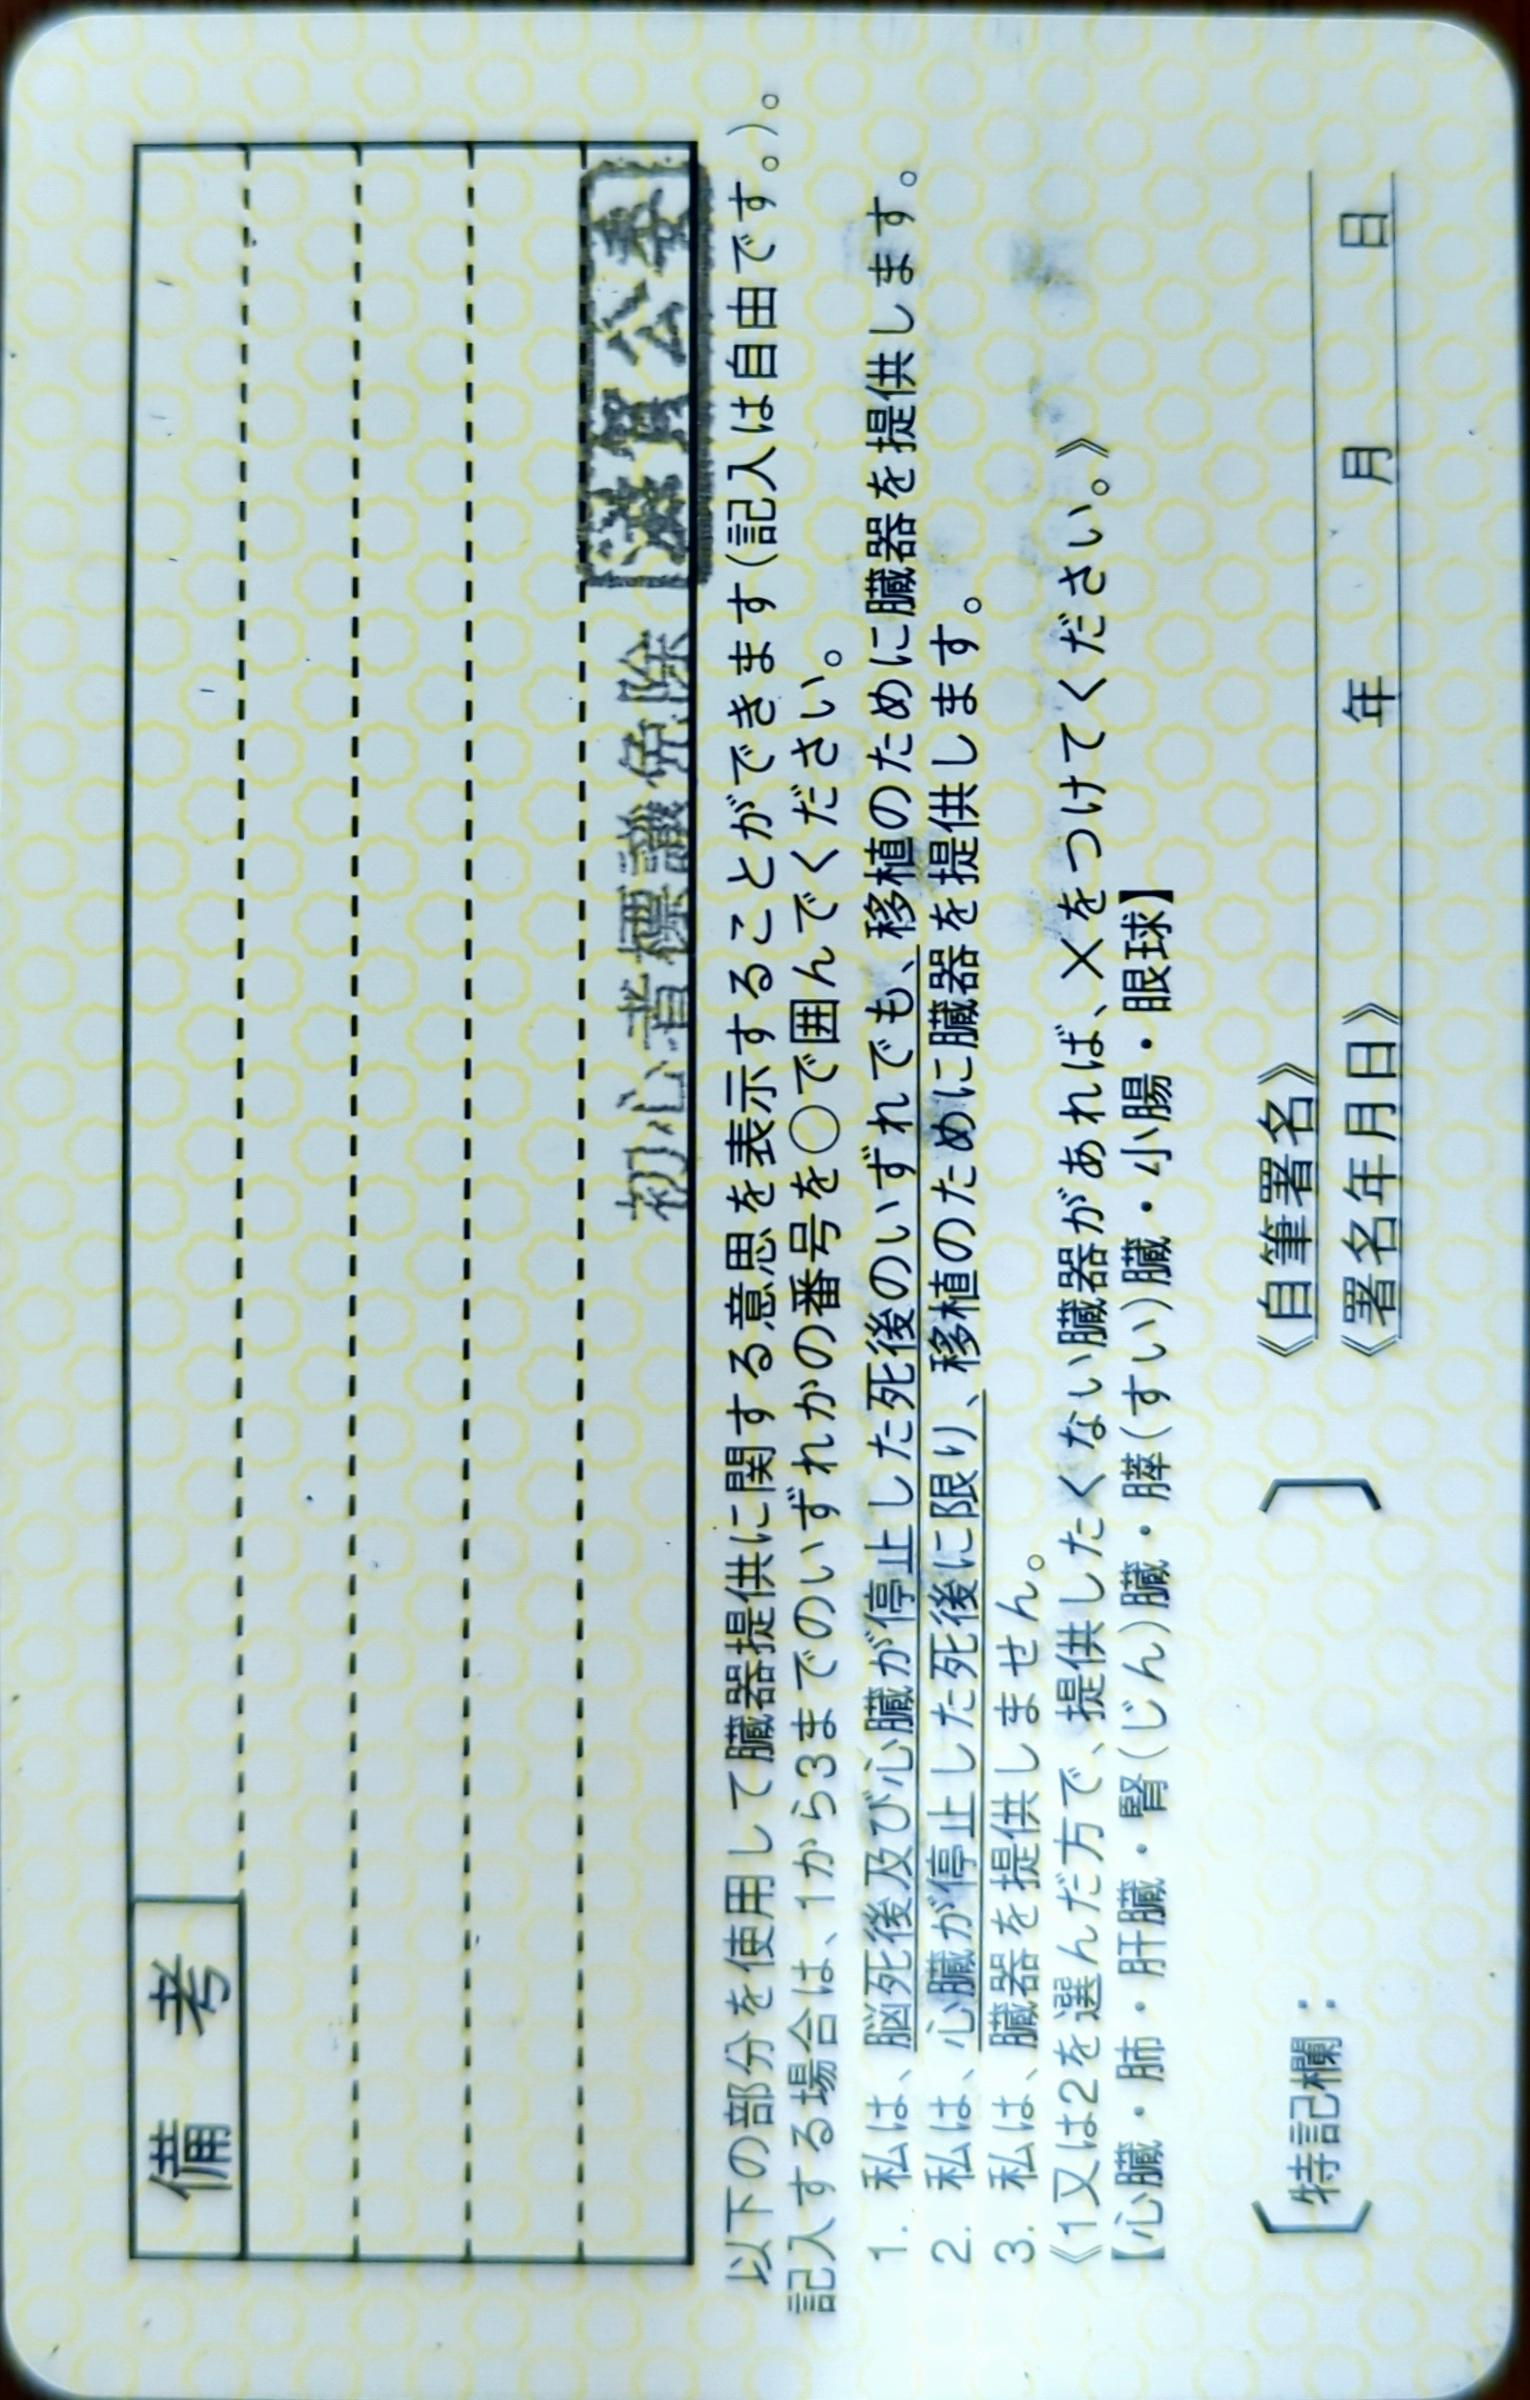
\includegraphics[width=40mm]{2022_05_27_1.jpg}
      \caption{Composite}
    \end{minipage}
    \begin{minipage}[b]{0.45\linewidth}
      \centering
      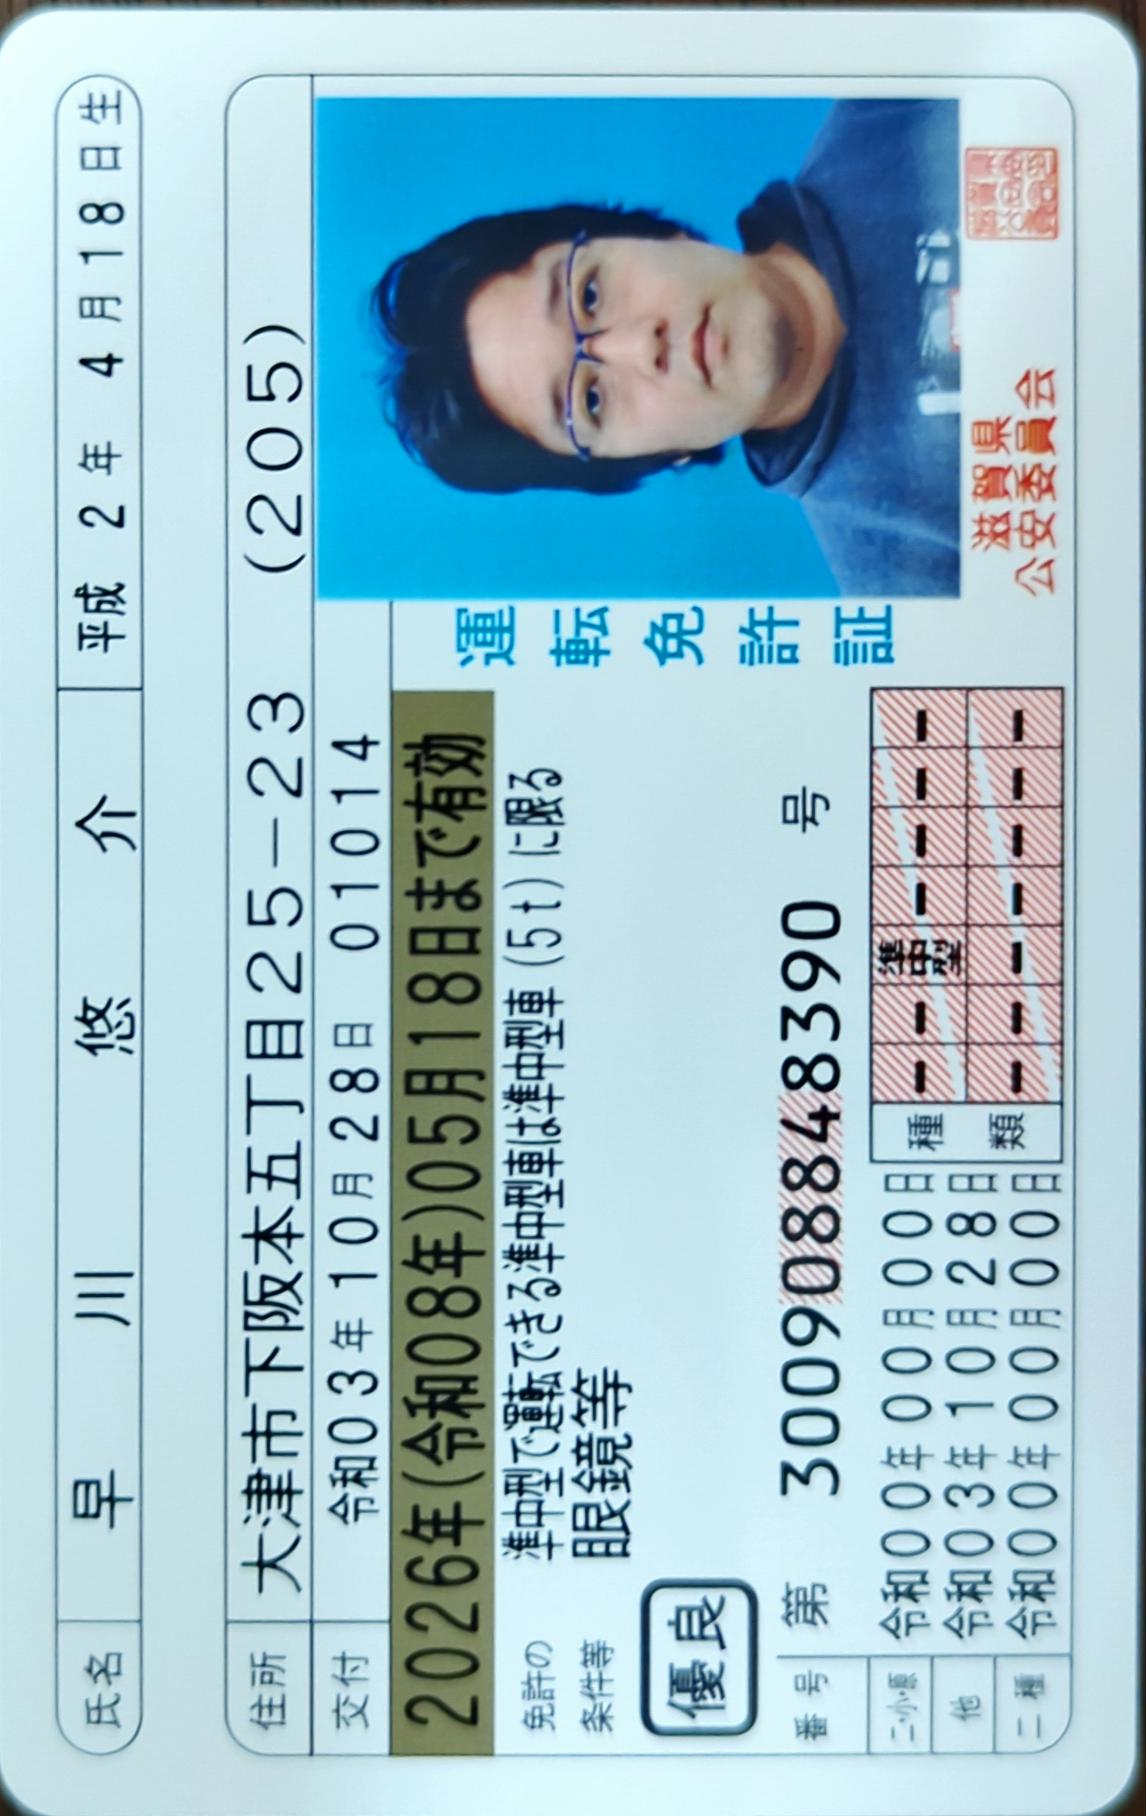
\includegraphics[width=40mm]{2022_05_27_2.jpg}
      \caption{Gradation}
    \end{minipage}
  \end{figure}

\end{document}